\documentclass[tikz,border=4pt]{standalone}
\usepackage{pgfplots}
\usepgfplotslibrary{groupplots}
\pgfplotsset{compat=1.18}
\begin{document}
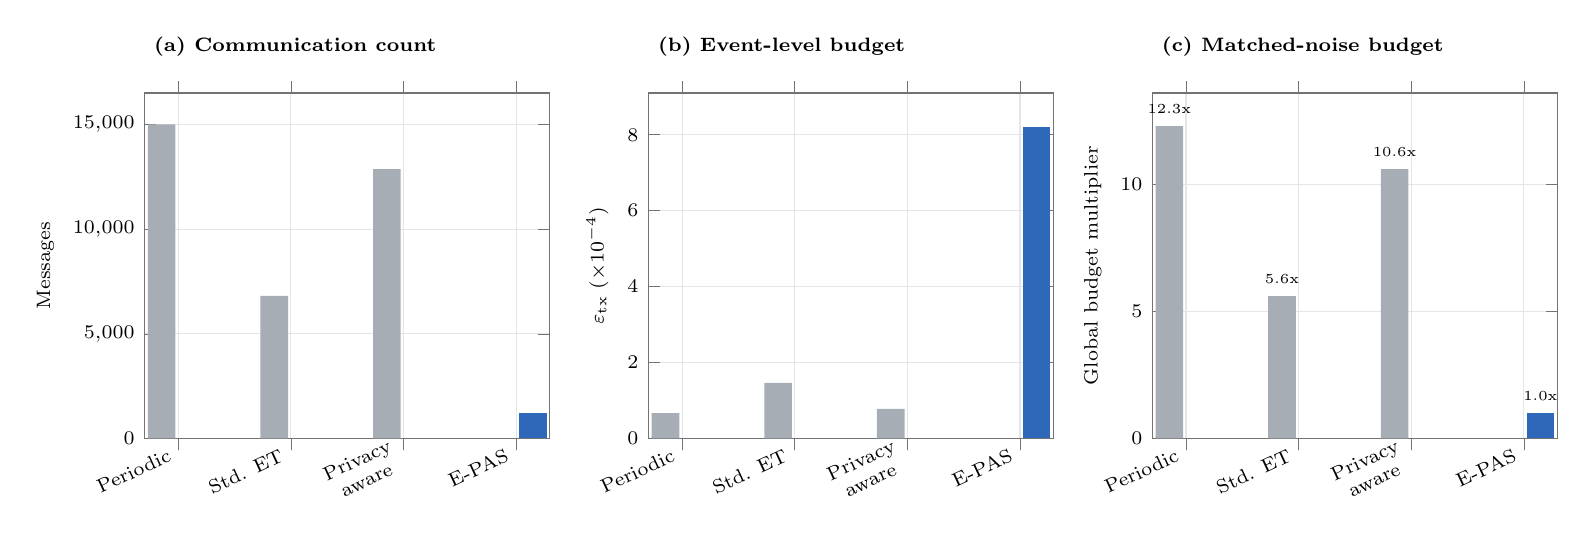
\begin{tikzpicture}
\definecolor{EBlue}{HTML}{2F68B8}
\definecolor{ENeutral}{HTML}{A7ADB5}
\begin{groupplot}[
  group style={group size=3 by 1, horizontal sep=1.25cm},
  width=2.65in,
  height=2.35in,
  ybar,
  ymin=0,
  tick label style={font=\scriptsize},
  label style={font=\scriptsize},
  title style={font=\scriptsize\bfseries, at={(0,1.03)}, anchor=south west},
  grid=major,
  major grid style={draw=black!10},
  axis line style={black!55},
  tick style={black!55},
  xtick={1,2,3,4},
  xticklabels={Periodic,Std. ET,Privacy\\aware,E-PAS},
  xticklabel style={align=center, rotate=25, anchor=east},
]
\nextgroupplot[
  title={(a) Communication count},
  ylabel={Messages},
  bar width=10pt,
  ymax=16500,
  scaled y ticks=false,
]
  \addplot[draw=none, fill=ENeutral] coordinates {(1,15000) (2,6814) (3,12863)};
  \addplot[draw=none, fill=EBlue] coordinates {(4,1218)};

\nextgroupplot[
  title={(b) Event-level budget},
  ylabel={$\varepsilon_{\mathrm{tx}}\;(\times 10^{-4})$},
  bar width=10pt,
  ymax=9.1,
]
  \addplot[draw=none, fill=ENeutral] coordinates {(1,0.667) (2,1.467) (3,0.777)};
  \addplot[draw=none, fill=EBlue] coordinates {(4,8.210)};

\nextgroupplot[
  title={(c) Matched-noise budget},
  ylabel={Global budget multiplier},
  bar width=10pt,
  ymax=13.6,
  nodes near coords,
  every node near coord/.append style={font=\tiny, yshift=1pt},
  point meta=explicit symbolic,
]
  \addplot[draw=none, fill=ENeutral] coordinates {(1,12.3) [12.3x] (2,5.6) [5.6x] (3,10.6) [10.6x]};
  \addplot[draw=none, fill=EBlue] coordinates {(4,1.0) [1.0x]};
\end{groupplot}
\end{tikzpicture}
\end{document}
